\chapter{系统设计}
\label{cha:design}

\section{设计目标与总体思路}
\label{sec:design_goal}

系统设计需要同时满足三类目标：一是保证企业私有知识在检索与问答过程中受到权限约束；二是保证文档从上传到知识可检索之间的处理链路清晰、可恢复、可扩展；三是保证最终用户能够以较低学习成本完成上传、检索和对话操作。

围绕上述目标，本文采用前后端分离、分层解耦和异步处理相结合的设计思路，将系统划分为表现层、接口与安全层、业务服务层以及数据与外部依赖层。该分层并非形式化拆分，而是为了在权限控制、长链路任务处理和交互响应之间建立清晰的职责边界。

在设计过程中，本文遵循几项彼此关联的原则，以保证架构描述、实现代码与系统边界保持一致。
\begin{enumerate}
    \item 权限语义必须先于具体功能建立，使文档上传、文件列表、检索召回、下载预览和问答生成等关键路径共享同一访问边界。
    \item 对于上传、解析、向量生成和索引写入等长链路任务，系统通过对象存储与消息队列降低耦合度，避免单个请求承担全部计算压力。
    \item 问答场景采用流式输出，上传场景保留分片续传与进度反馈，使用户能够持续感知任务状态。
\end{enumerate}

\section{总体架构设计}
\label{sec:overall_design}

系统总体架构如图 \ref{fig:system-architecture} 所示。前端以知识库页面、聊天页面、组织标签页面和用户管理页面为主要入口；后端以 Spring Boot 应用为核心，负责认证授权、文档处理、检索问答和会话管理。

数据层由 MySQL、Redis、MinIO 与 Elasticsearch 共同构成，外部能力则通过大模型接口、嵌入接口和 Kafka 消息中间件接入。多组件协同是系统设计的基本前提：关系型存储负责业务状态，对象存储负责文件实体，搜索引擎负责知识检索，消息队列负责将上传请求与计算密集型处理过程解耦。

\begin{figure}[H]
    \centering
    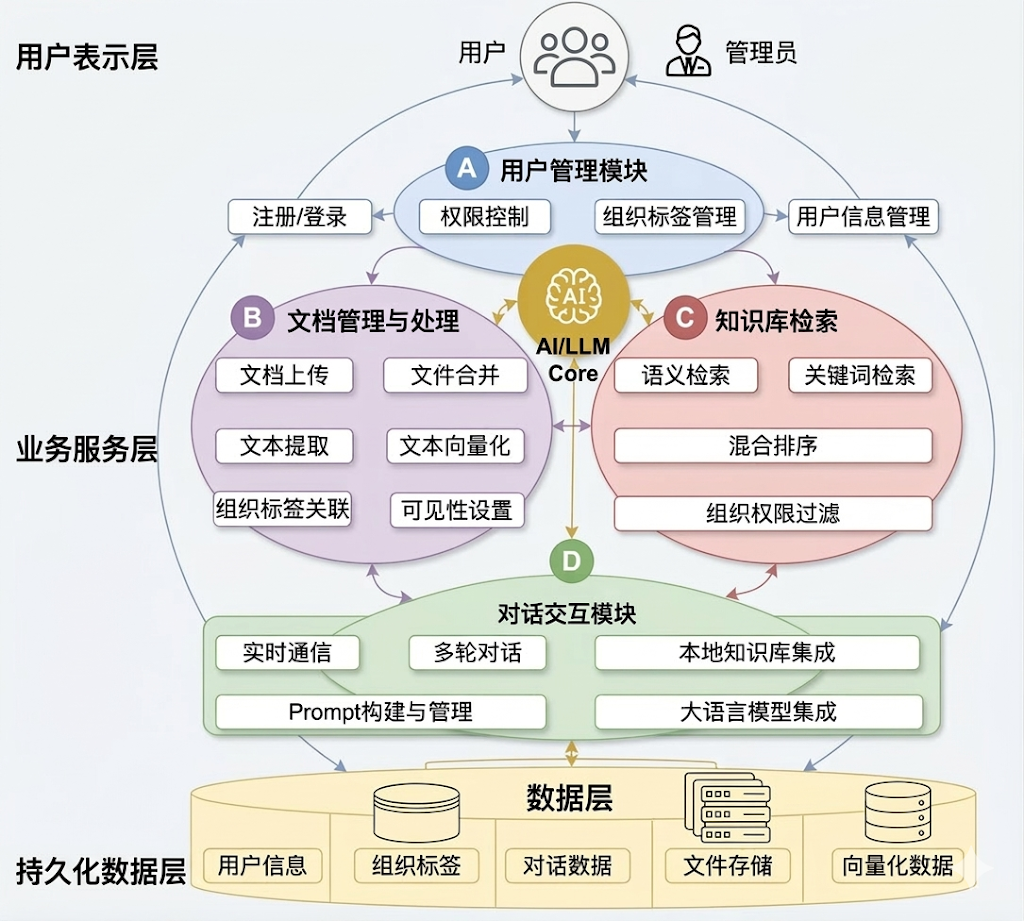
\includegraphics[width=0.82\textwidth]{image/chap03/structure.png}
    \caption{系统总体架构图}
    \label{fig:system-architecture}
\end{figure}

表现层由 Vue 3、TypeScript 与 Vite 组成，负责文件上传、文件列表管理、知识检索、聊天问答、用户信息展示和组织标签维护等界面交互。

接口与安全层由 RESTful API、WebSocket 通道以及 Spring Security 相关过滤器构成，主要承担请求接入、身份识别和组织授权。

业务服务层围绕用户管理、文档上传、文档解析、向量化、混合检索、会话管理和文件服务展开，负责实现核心业务逻辑。

数据与外部依赖层则由 MySQL、Redis、MinIO、Elasticsearch、DeepSeek 接口和 Kafka 共同组成，对应状态持久化、对象存储、知识检索、模型调用和异步解耦等职责。

\subsection{技术选型}

表 \ref{tab:tech-stack} 汇总了本系统的核心技术组件及其选择原因。

\begin{table}[H]
    \centering
    \caption{核心技术选型}
    \label{tab:tech-stack}
    {\footnotesize
    \begin{tabular}{L{1.8cm}L{3.0cm}L{8.0cm}}
        \toprule
        层次 & 技术组件 & 选择原因 \\
        \midrule
        前端框架 & \makecell[l]{Vue 3、\\TypeScript、Vite} & Vue 3 采用组件化开发方式，适合构建知识库、问答与管理页面等多视图交互界面；TypeScript 有助于约束前后端接口数据结构，降低维护成本；Vite 在开发阶段启动快、热更新响应及时，适合需要频繁迭代的前端工程。 \\
        后端框架 & \makecell[l]{Spring Boot 3.4.2、\\Java 17} & Spring Boot 生态成熟，便于统一组织接口层、服务层和配置管理；Java 17 作为长期支持版本，兼顾稳定性、性能与工程可维护性，适合承载企业知识系统的核心业务逻辑。 \\
        安全机制 & \makecell[l]{Spring Security、\\JWT} & Spring Security 提供完整的过滤器链与授权扩展能力，便于把角色和组织标签约束整合到统一认证流程中；JWT 适合前后端分离场景下的无状态认证，能够减少服务端会话管理负担。 \\
        文件存储 & MinIO & MinIO 兼容 S3 接口，便于实现分片上传、对象合并和预签名访问；同时其私有化部署成本较低，更符合企业内部文档系统对数据可控性的要求。 \\
        数据存储 & \makecell[l]{MySQL、Redis、\\Elasticsearch} & MySQL 适合保存用户、组织标签和文件元数据等结构化信息；Redis 读写延迟低，适合缓存上传状态和会话数据；Elasticsearch 同时支持全文检索与向量检索，适合构建权限约束下的混合检索能力。 \\
        异步处理 & Kafka & 文件解析、切分和向量化属于耗时较长的后台任务，Kafka 能够在上传完成后将请求链路与入库链路解耦，并通过消息缓冲提高系统在高并发场景下的稳定性。 \\
        文档处理 & Apache Tika、HanLP & Apache Tika 支持多种文档格式的统一文本提取，能够减少不同文件类型的解析差异；HanLP 对中文分词和长句切分支持较好，适合后续语义切分与检索片段构建。 \\
        模型调用 & \makecell[l]{DeepSeek API、\\Embedding API} & 系统需要同时具备文本生成与向量表示能力，因此分别选用对话模型接口和嵌入接口；该组合便于将生成链路与检索链路分开设计，也更利于后续模型替换与能力扩展。 \\
        \bottomrule
    \end{tabular}
    }
\end{table}

\section{核心模块设计}
\label{sec:core_design}

在总体架构确定之后，选取权限控制、文档入库、混合检索和对话编排四条直接影响系统行为的主链路展开设计说明。

\subsection{权限模型与多租户隔离设计}
\label{sec:permission_design}

系统的权限模型不是单纯的角色控制，而是由“角色、主组织标签、组织标签集合、文档公开性、文档归属者”共同决定。管理员可以访问和维护系统内全部资源。每个用户在注册时都会自动生成一个私人组织标签，并以此构建个人私有空间。普通用户可以访问自己上传的文档、公开文档以及组织标签匹配的共享文档。对于检索和文件列表查询，系统还需要根据组织标签层级展开用户的有效标签集合，以允许用户访问父级组织范围内的共享文档。

权限映射关系如图 \ref{fig:permission-mapping} 所示。该设计的关键不在于“是否有某个角色”，而在于如何将用户身份信息映射为后续数据访问阶段可直接使用的过滤条件。角色只是权限计算的起点；真正进入检索与文件服务阶段时，起作用的是用户可见组织范围、文档归属关系与公开属性的组合结果。

\begin{figure}[H]
    \centering
    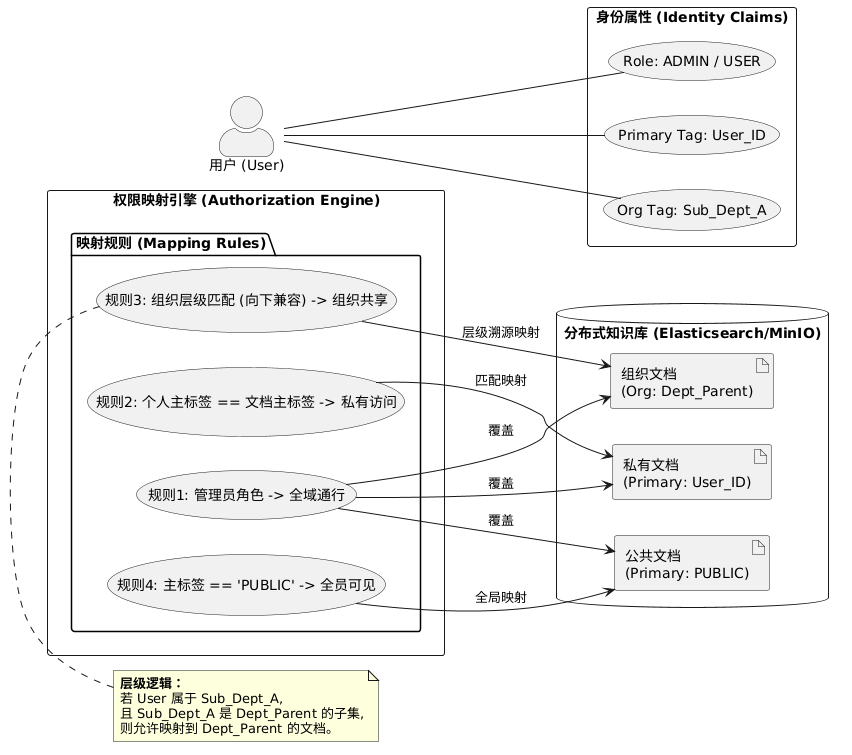
\includegraphics[width=0.72\textwidth]{image/chap03/org.png}
    \caption{权限映射关系图}
    \label{fig:permission-mapping}
\end{figure}

当用户发起文件访问或检索请求时，系统按图 \ref{fig:permission-decision} 的逻辑完成权限判断。代码中资源级过滤器以快速拦截为主，检索服务和文件列表服务则结合缓存服务计算用户有效标签集合，并完成更完整的层级权限展开，两者共同构成系统的多租户隔离机制。

\begin{figure}[H]
    \centering
    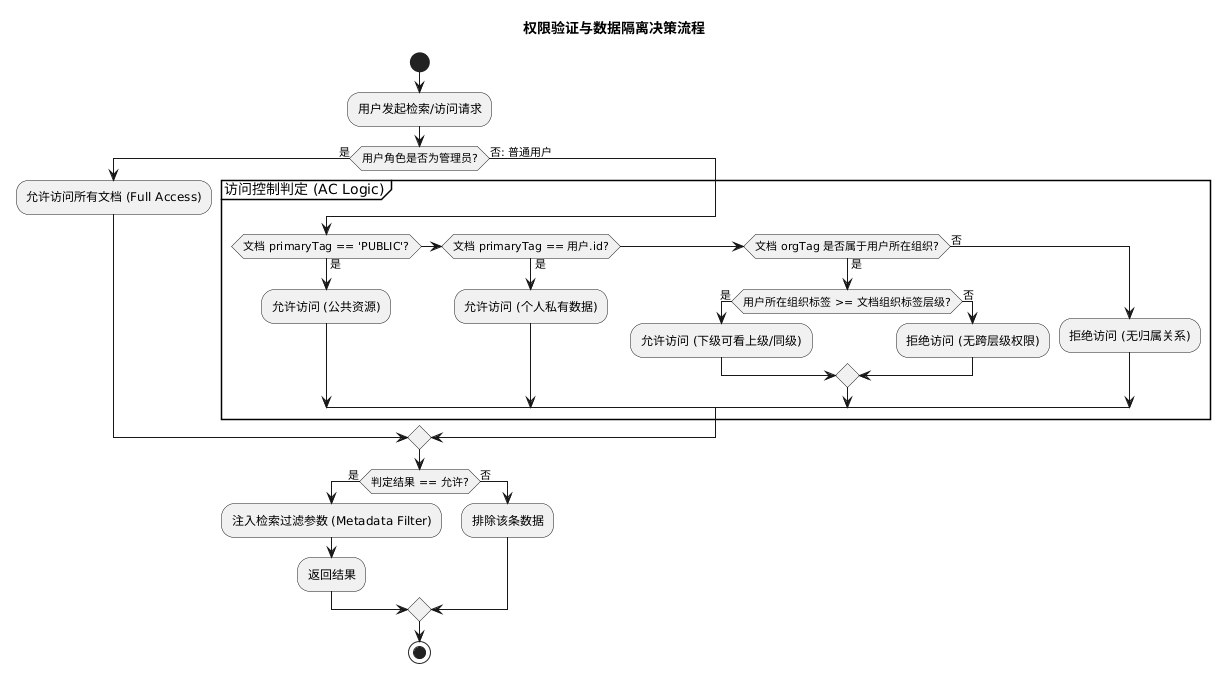
\includegraphics[width=0.95\textwidth]{image/chap03/acc.png}
    \caption{权限判定与数据隔离流程图}
    \label{fig:permission-decision}
\end{figure}

\subsection{文档接入与知识入库链路设计}
\label{sec:document_pipeline_design}

文档接入链路是连接“原始文件”与“知识索引”的关键桥梁。如图~\ref{fig:document-pipeline}所示，系统先在前端对待上传文件执行 MD5 计算并按固定粒度切分，再逐片提交上传请求。后端接收分片后，在 MySQL 中维护文件记录，在 Redis 中维护分片位图，并将分片对象写入 MinIO。

全部分片上传完成后，服务端依据文件 MD5 对应的分片列表完成对象合并并写回文件状态。随后，控制器将文件处理任务发送至 Kafka，由消费者在后台执行文档解析与向量化。解析服务负责将文本切分结果写入关系型存储，向量化服务再将文本分块与向量写入 Elasticsearch 知识索引。由此，文件从“已上传”转化为“可检索知识”的过程被明确拆分为传输、状态确认、后台处理和索引写入四个阶段。

该链路的设计重点是将“上传可靠性”和“入库吞吐量”分开考虑。文件上传阶段更关注状态恢复和数据完整性，后台解析与向量化阶段则更强调计算密集任务的异步化处理。如果将两类职责压缩进单次请求，系统会同时承担传输、解析与索引写入压力，既不利于错误恢复，也不利于后续扩展。

\begin{figure}[H]
    \centering
    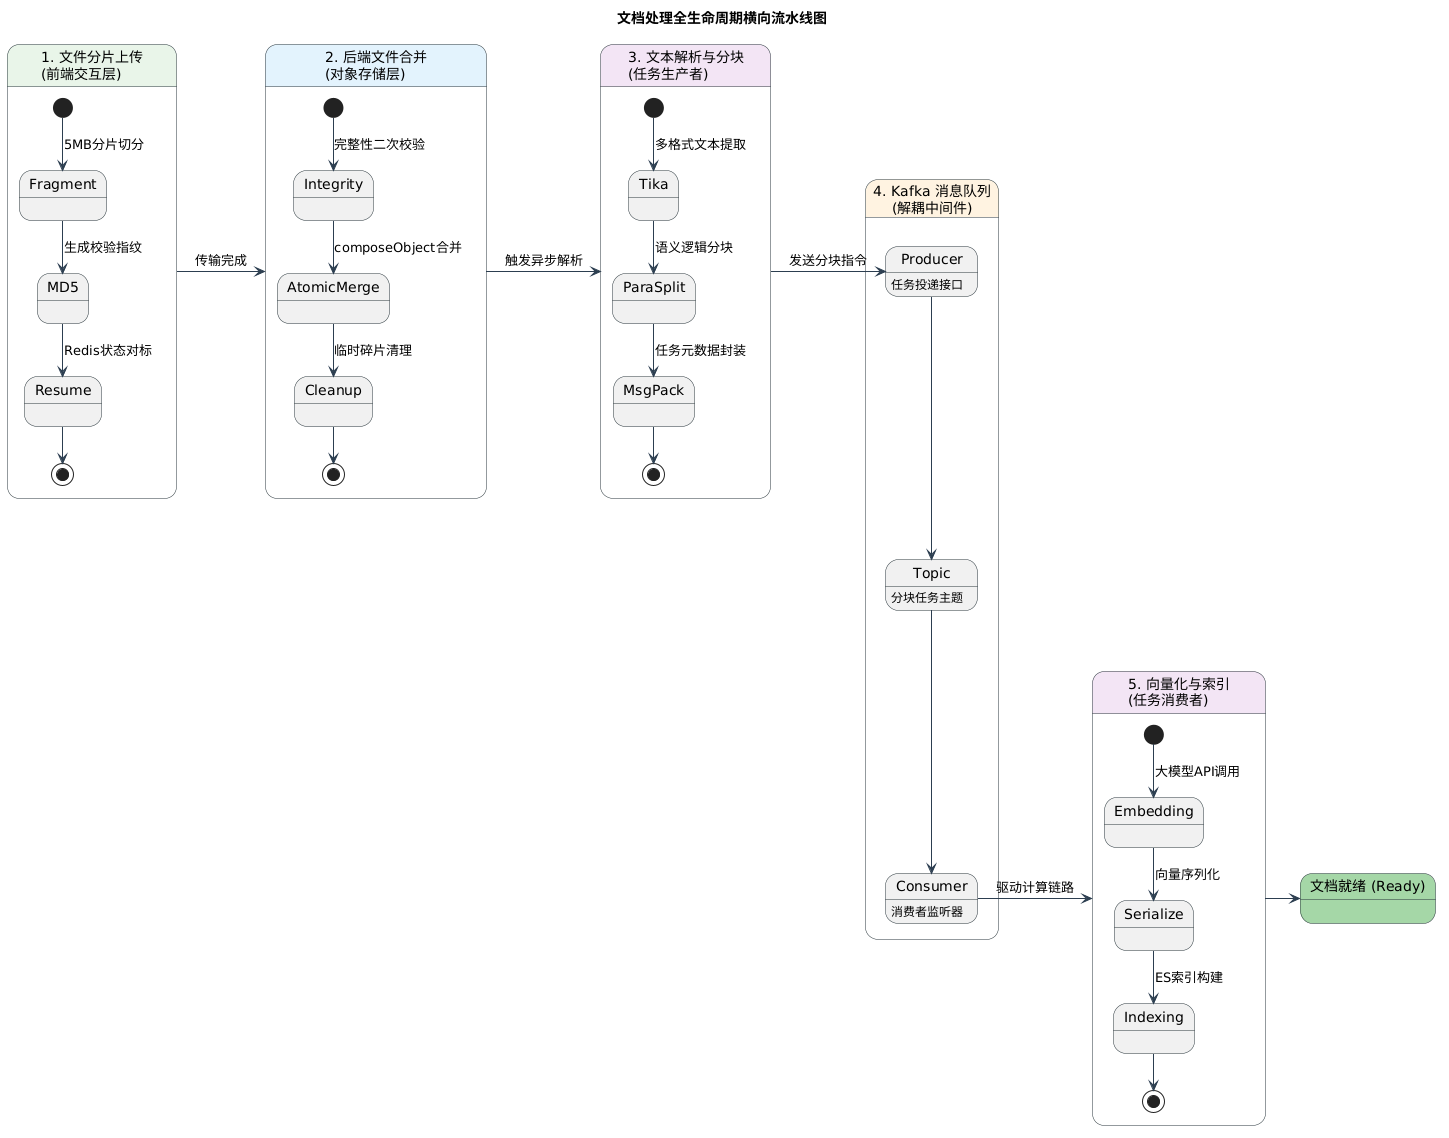
\includegraphics[width=0.98\textwidth]{image/chap03/text.png}
    \caption{文档处理全生命周期设计图}
    \label{fig:document-pipeline}
\end{figure}

\subsection{混合检索设计}
\label{sec:retrieval_design}

为兼顾企业文档场景中的术语匹配能力与语义泛化能力，系统采用“语义召回+文本重排+权限过滤”的混合检索设计。这里的出发点是希望在专业文档场景中同时保留语义相近性判断与术语精确定位能力。因为单一检索路径在不同任务中容易出现召回偏移，检索效果还会受到候选组织方式与后续编排方式的共同影响\cite{rahman2025comparative}。因此，企业知识场景中的检索设计不能只追求“语义上相似”，还必须考虑候选结果是否便于后续验证与生成使用。

为此，系统进行两阶段混合检索设计。在第一阶段使用嵌入模型将用户问题转换为查询向量，并执行 kNN 召回；与此同时，将用户身份、公开属性和组织标签约束作为过滤条件一并注入查询，避免未授权文档进入候选集。在第二阶段，系统对候选结果执行文本匹配重排序，使包含关键术语、编号或精确表述的片段获得更高优先级。权限过滤被放置在召回阶段共同执行，而不是放到结果返回后再处理，从而保证检索执行过程中的事实一致性、结果可核对性和安全边界。

混合检索与安全过滤的总体流程如图~\ref{fig:hybrid-retrieval-design}所示。

\begin{figure}[H]
    \centering
    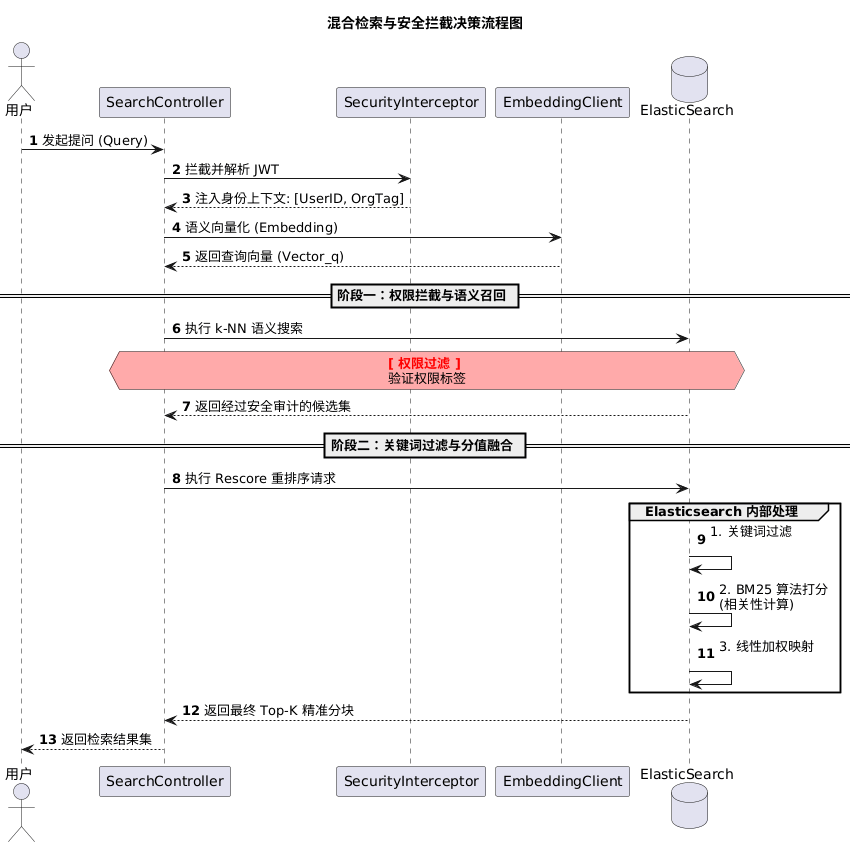
\includegraphics[width=0.78\textwidth]{image/chap03/retrive.png}
    \caption{混合检索与安全过滤设计图}
    \label{fig:hybrid-retrieval-design}
\end{figure}

\subsection{对话编排与生成设计}
\label{sec:generation_design}

问答模块以“检索结果受约束的生成”为核心。系统在会话阶段并不直接将用户问题发送给模型，而是先确定当前用户的会话状态，再决定哪些外部证据能够进入生成过程。这样的设计并不是简单把“检索”和“生成”顺序连接起来，而是把提示词组织本身视为知识治理链路的一部分。企业知识管理研究指出，提示编排不仅影响回答形式，也会影响知识在系统中的组织与调用方式\cite{oleary2024km}。因此，在企业场景下，生成阶段同样需要接受上下文边界、来源组织方式和会话连续性的共同约束。

基于上述约束，系统先从 Redis 读取当前用户会话标识及历史消息，再调用混合检索服务获取带来源编号的候选知识片段。随后，系统将规则、检索结果、历史对话和本轮问题拼接为标准化提示词，最后再调用对话模型接口以流式方式逐段返回生成内容。

在这一编排过程中，本轮问题及历史消息保障问答的连续性。但是回答质量也不能只看流畅性，还需要与风险控制和适用边界同时衡量\cite{liang2023holistic}，因此规则约束用于限制模型偏离检索证据或暴露敏感信息。而来源编号则用于保留可追溯的证据链，因为外部证据约束是提高回答可信度的重要条件\cite{zhang2025hallucination}，特别对于垂直领域知识问答，检索结果的可解释性和可核对性同样重要\cite{tcmstandardrag2025}。

提示词编排与生成流程如图~\ref{fig:generation-design}所示。

\begin{figure}[H]
    \centering
    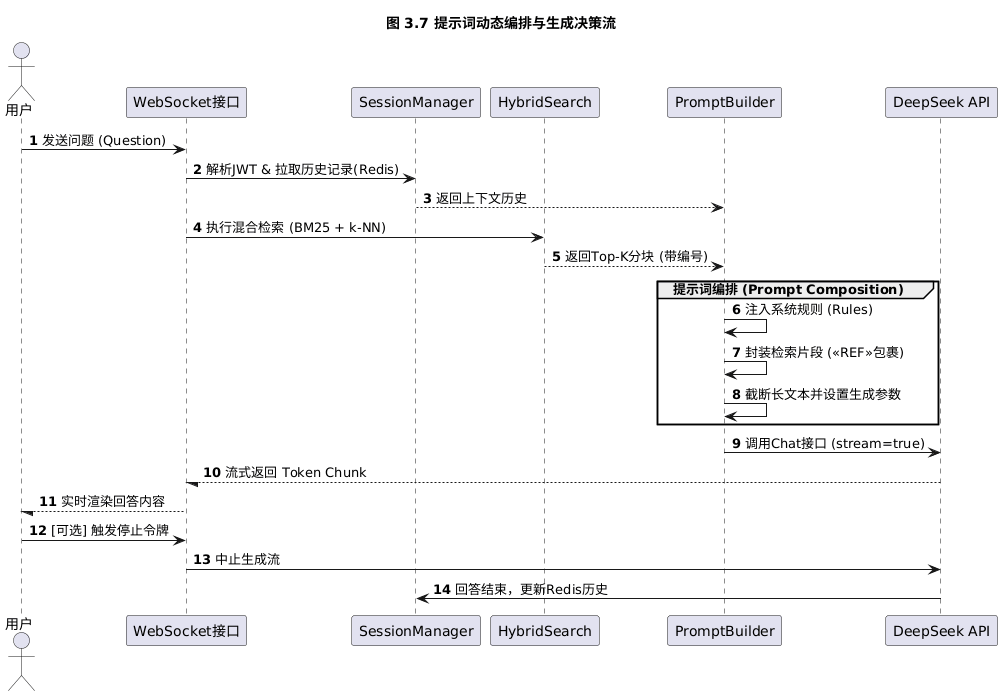
\includegraphics[width=0.92\textwidth]{image/chap03/generate.png}
    \caption{提示词编排与生成流程图}
    \label{fig:generation-design}
\end{figure}

\section{数据结构设计}
\label{sec:data_design}

数据结构设计的作用并不只是给表和字段命名，更重要的是让权限信息、处理状态和检索结果能够在多种存储之间连续传递。考虑到系统同时使用关系型数据库、对象存储与搜索引擎，本节分别说明业务元数据和知识索引的组织方式，以及它们如何共同支撑后续实现。

\subsection{关系型存储结构}

系统在关系型数据库中主要维护用户、组织标签、文件上传记录、分片记录和文本分块记录。五个实体之间的关系如图 \ref{fig:er-diagram} 所示。

\begin{figure}[H]
    \centering
    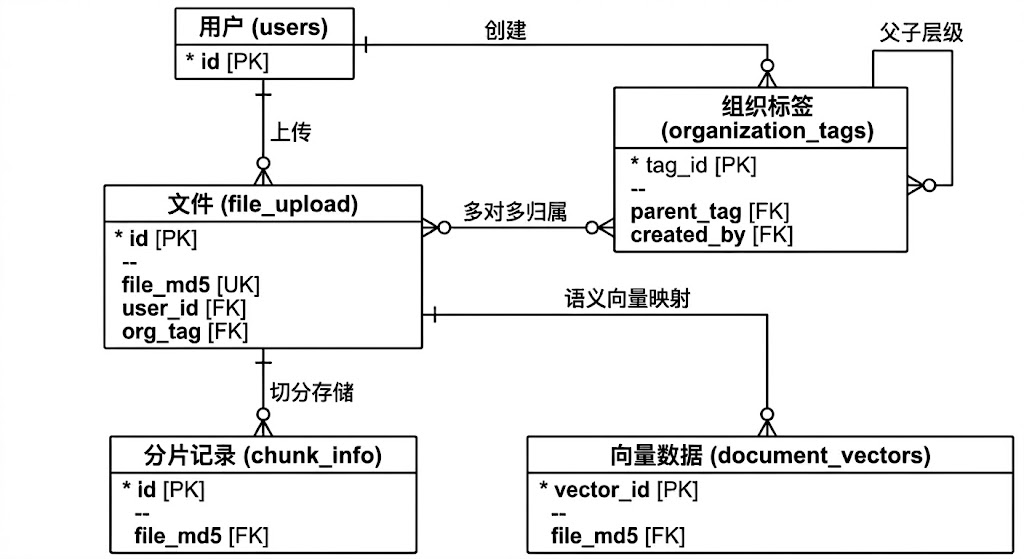
\includegraphics[width=0.92\textwidth]{image/chap03/ER.png}
    \caption{系统 E-R 图}
    \label{fig:er-diagram}
\end{figure}

在实体关系基础上，核心关系表的字段设计及其作用说明如表 \ref{tab:relational-objects} 所示。

\begin{table}[H]
    \centering
    \caption{关系型核心存储对象设计}
    \label{tab:relational-objects}
    {\footnotesize
    \newcommand{\relcell}[1]{\parbox[c][1.3cm][c]{\linewidth}{\raggedright\strut #1\strut}}
    \begin{tabular}{L{2.35cm}L{4.15cm}L{6.2cm}}
        \toprule
        存储对象 & 关键字段 & 作用说明 \\
        \midrule
        \relcell{\texttt{users}} & \relcell{\texttt{id}、\texttt{username}、\texttt{role}、\texttt{org\_tags}、\texttt{primary\_org}} & \relcell{保存用户身份、角色及组织标签信息，是认证授权与界面展示的基础数据} \\
        \relcell{{\scriptsize \texttt{organization}}\\{\scriptsize \texttt{\_tags}}} & \relcell{\texttt{tag\_id}、\texttt{name}、\texttt{parent\_tag}、\texttt{created\_by}} & \relcell{保存组织标签及其层级关系，为组织共享范围和有效标签展开提供依据} \\
        \relcell{\texttt{file\_}\\\texttt{upload}} & \relcell{\texttt{file\_md5}、\texttt{fileName}、\texttt{user\_id}、\texttt{org\_tag}、\texttt{is\_public}、\texttt{status}} & \relcell{保存文件级元数据、归属关系与上传状态，是文件服务与权限校验的入口对象} \\
        \relcell{\texttt{chunk\_}\\\texttt{info}} & \relcell{\texttt{fileMd5}、\texttt{chunkIndex}、\texttt{chunkMd5}、\texttt{storagePath}} & \relcell{记录上传分片信息，支撑断点续传和服务端对象合并} \\
        \relcell{\texttt{document\_}\\\texttt{vectors}} & \relcell{\texttt{vectorId}、\texttt{fileMd5}、\texttt{chunkId}、\texttt{textContent}、\texttt{user\_id}、\texttt{org\_tag}} & \relcell{保存解析后的文本分块及其权限元数据，作为向量化写入前的中间结果} \\
        \bottomrule
    \end{tabular}
    }
\end{table}

\subsection{知识索引结构}

由于 Elasticsearch 的特性，系统将文本分块与向量结果共同写入 Elasticsearch 索引 \texttt{knowledge\_base}。该索引结构如表 \ref{tab:es-fields} 所示。

\begin{table}[H]
    \centering
    \caption{Elasticsearch 知识索引字段设计}
    \label{tab:es-fields}
    {\footnotesize
    \begin{tabularx}{\textwidth}{L{2.5cm}L{2.1cm}Y}
        \toprule
        字段名 & 类型 & 作用说明 \\
        \midrule
        \texttt{fileMd5} & \texttt{keyword} & 关联原始文件标识，用于结果回填与删除同步 \\
        \texttt{chunkId} & \texttt{integer} & 标识文件内的分块序号 \\
        \makecell[l]{\texttt{text}\\\texttt{Content}} & \texttt{text} & 保存可检索文本内容，并配置中文分词器用于全文匹配 \\
        \texttt{vector} & \makecell[l]{\texttt{dense\_}\\\texttt{vector}} & 保存 2048 维嵌入向量，用于 kNN 语义检索 \\
        \makecell[l]{\texttt{model}\\\texttt{Version}} & \texttt{keyword} & 标识生成向量所使用的模型版本 \\
        \texttt{userId} & \texttt{keyword} & 标识上传者，用于权限过滤和结果展示 \\
        \texttt{orgTag} & \texttt{keyword} & 标识文档所属组织标签，用于检索阶段过滤 \\
        \texttt{isPublic} & \texttt{boolean} & 标识公开属性，用于跨用户共享资源判断 \\
        \bottomrule
    \end{tabularx}
    }
\end{table}

上述设计使系统形成了“关系型数据库负责业务元数据、对象存储负责原始文件、搜索引擎负责知识检索”的多存储协同结构，为后续实现章节中的关键代码提供了清晰的数据基础。
